\documentclass[tikz,border=10pt]{standalone}
\usepackage{amsmath}
\usetikzlibrary{arrows.meta}
\definecolor{ink}{HTML}{21352F}
\definecolor{teal}{HTML}{087F7B}
\definecolor{blue}{HTML}{4B77A8}
\definecolor{gold}{HTML}{C58B2A}

\begin{document}
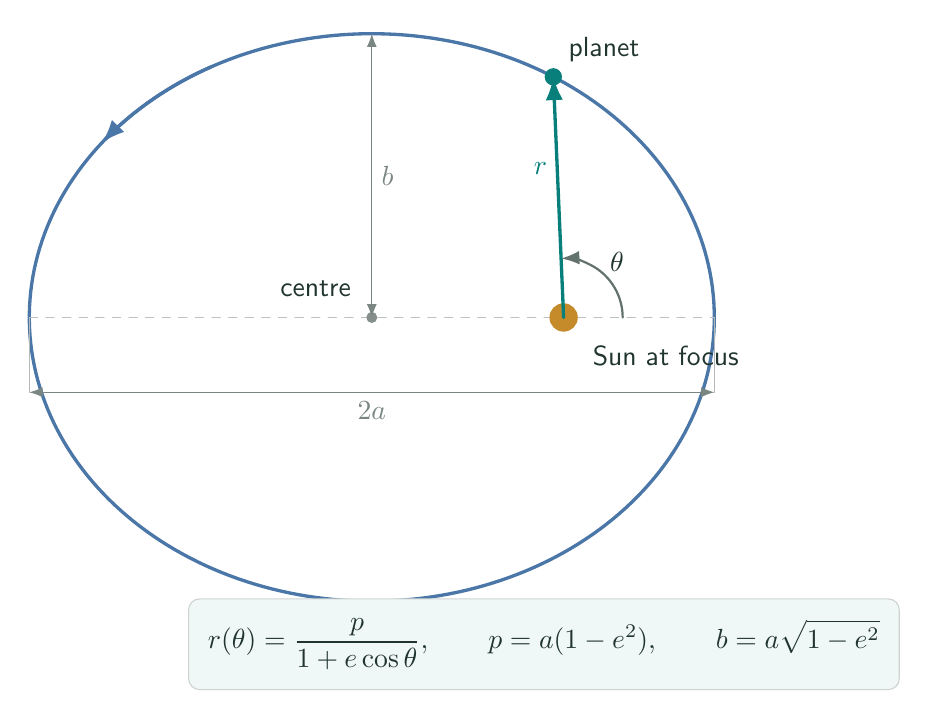
\begin{tikzpicture}[font=\sffamily,text=ink,>=Latex,line cap=round,line join=round]
  \pgfmathsetmacro{\smajor}{4.35}
  \pgfmathsetmacro{\ecc}{0.56}
  \pgfmathsetmacro{\sminor}{\smajor*sqrt(1-\ecc*\ecc)}
  \pgfmathsetmacro{\focusdist}{\smajor*\ecc}
  \pgfmathsetmacro{\semilatus}{\smajor*(1-\ecc*\ecc)}

  % The Sun is the right-hand focus at the origin; the ellipse centre is (-ae,0).
  \draw[blue,very thick]
    plot[domain=0:360,samples=240,variable=\t]
      ({\smajor*cos(\t)-\focusdist},{\sminor*sin(\t)});
  \draw[blue,very thick,->]
    plot[domain=118:142,samples=30,variable=\t]
      ({\smajor*cos(\t)-\focusdist},{\sminor*sin(\t)});

  \draw[ink!30,dashed]
    ({-\smajor-\focusdist},0)--({\smajor-\focusdist},0);
  \coordinate (C) at (-\focusdist,0);
  \fill[ink!55] (C) circle (0.07);
  \node[above left=4pt] at (C) {centre};

  \coordinate (S) at (0,0);
  \fill[gold] (S) circle (0.18);
  \node[below right=7pt] at (S) {Sun at focus};

  \pgfmathsetmacro{\Epoint}{58}
  \pgfmathsetmacro{\px}{\smajor*cos(\Epoint)-\focusdist}
  \pgfmathsetmacro{\py}{\sminor*sin(\Epoint)}
  \pgfmathsetmacro{\polarangle}{atan2(\py,\px)}
  \coordinate (P) at (\px,\py);
  \fill[teal] (P) circle (0.11);
  \node[above right=2pt] at (P) {planet};
  \draw[teal,very thick,->] (S)--(P)
    node[pos=.55,above left] {$r$};
  \draw[ink!70,thick,->] (0.75,0)
    arc[start angle=0,end angle=\polarangle,radius=.75];
  \node at ({.98*cos(\polarangle/2)},{.98*sin(\polarangle/2)}) {$\theta$};

  \draw[ink!35]
    ({-\smajor-\focusdist},0)--({-\smajor-\focusdist},-.95);
  \draw[ink!35]
    ({\smajor-\focusdist},0)--({\smajor-\focusdist},-.95);
  \draw[<->,ink!60]
    ({-\smajor-\focusdist},-.95)--({\smajor-\focusdist},-.95)
    node[midway,below] {$2a$};
  \draw[<->,ink!60]
    (-\focusdist,0)--(-\focusdist,\sminor)
    node[midway,right] {$b$};

  \node[draw=ink!22,rounded corners=4pt,fill=teal!6,inner sep=7pt]
    at (-.25,-4.15)
    {$\displaystyle r(\theta)=\frac{p}{1+e\cos\theta},\qquad
      p=a(1-e^2),\qquad b=a\sqrt{1-e^2}$};
\end{tikzpicture}
\end{document}
